%%=============================================================================
%% LaTeX sjabloon voor bachelorproef, HoGent Bedrijf en Organisatie
%% Opleiding Toegepaste Informatica
%%=============================================================================

\documentclass[fleqn,a4paper,12pt]{book}

%%=============================================================================
%% LaTeX sjabloon voor de bachelorproef, HoGent Bedrijf en Organisatie
%% Opleiding toegepaste informatica
%%
%% Structuur en algemene vormgeving. Meestal hoef je hier niets te wijzigen.
%%
%% Vormgeving gebaseerd op "The Legrand Orange Book", version 2.0 (9/2/15)
%% door Mathias Legrand (legrand.mathias@gmail.com) met aanpassingen door
%% Vel (vel@latextemplates.com). Het oorspronkelijke template is te vinden op
%% http://www.LaTeXTemplates.com
%%
%% Aanpassingen voor HoGent toegepaste informatica: 
%%   Bert Van Vreckem <bert.vanvreckem@hogent.be>
%% Licentie: 
%%   CC BY-NC-SA 3.0 (http://creativecommons.org/licenses/by-nc-sa/3.0/)
%%=============================================================================

\nonstopmode

\usepackage{longtable}
\usepackage[acronym]{glossaries}
\usepackage{listings}  
\usepackage[final]{pdfpages}
\usepackage{scrextend}
\usepackage{listings} %For code in appendix
\lstset
{ %Formatting for code in appendix
    language=Matlab,
    basicstyle=\footnotesize,
    numbers=left,
    stepnumber=1,
    showstringspaces=false,
    tabsize=1,
    breaklines=true,
    breakatwhitespace=false,
}
\usepackage[acronym,xindy]{glossaries}

\makeglossaries

%%-----------------------------------------------------------------------------
%% Packages
%%-----------------------------------------------------------------------------

\usepackage[top=3cm,bottom=3cm,left=3cm,right=3cm,headsep=10pt,a4paper]{geometry} % Page margins
\usepackage[utf8]{inputenc}  % Accenten gebruiken in tekst (vb. é ipv \'e)
\usepackage{amsfonts}        % AMS math packages: extra wiskundige
\usepackage{amsmath}         %   symbolen (o.a. getallen-
\usepackage{amssymb}         %   verzamelingen N, R, Z, Q, etc.)
\usepackage[english,dutch]{babel}    % Taalinstellingen: woordsplitsingen,
                             %  commando's voor speciale karakters
                             %  ("dutch" voor NL)
\usepackage{iflang}
\usepackage{eurosym}         % Euro-symbool €
\usepackage{geometry}
\usepackage{graphicx}        % Invoegen van tekeningen
\graphicspath{{img/}}       % Specifies the directory where pictures are stored
\usepackage{tikz}            % Required for drawing custom shapes
\usepackage[pdftex,bookmarks=true]{hyperref}
                             % PDF krijgt klikbare links & verwijzingen,
                             %  inhoudstafel
\usepackage{enumitem}        % Customize lists
\setlist{nolistsep}         % Reduce spacing between list items
\usepackage{listings}        % Broncode mooi opmaken
\usepackage{multirow}        % Tekst over verschillende cellen in tabellen
\usepackage{rotating}        % Tabellen en figuren roteren

\usepackage{booktabs}        % Required for nicer horizontal rules in tables

\usepackage{xcolor}          % Required for specifying colors by name
\definecolor{maincolor}{RGB}{0,147,208} % Define the main color used for 
                             % highlighting throughout the book
                             % 0, 147, 208 = officiële kleur HoGent FBO

% Paragraph style: no indent, add space between paragraphs
\setlength{\parindent}{0em}
\setlength{\parskip}{1em}

\usepackage{etoolbox}
\usepackage{titling} % Macros for title, author, etc
\usepackage{lipsum}          % Voor vultekst (lorem ipsum)
\usepackage{underscore} % make it possible to use _ in your text

%----------------------------------------------------------------------------------------
%	FONTS
%----------------------------------------------------------------------------------------

\usepackage{avant} % Use the Avantgarde font for headings
%\usepackage{times} % Use the Times font for headings
\usepackage{mathptmx} % Use the Adobe Times Roman as the default text font together with math symbols from the Sym­bol, Chancery and Com­puter Modern fonts

\usepackage{microtype} % Slightly tweak font spacing for aesthetics
\usepackage[utf8]{inputenc} % Required for including letters with accents
\usepackage[T1]{fontenc} % Use 8-bit encoding that has 256 glyphs

%------------------------------------------------------------------------------
%	TITLE PAGE
%------------------------------------------------------------------------------

\newcommand{\inserttitlepage}{%
\begin{titlepage}
  \newgeometry{top=2cm,bottom=1.5cm,left=1.5cm,right=1.5cm}
  \begin{center}

    \begingroup
    \rmfamily
    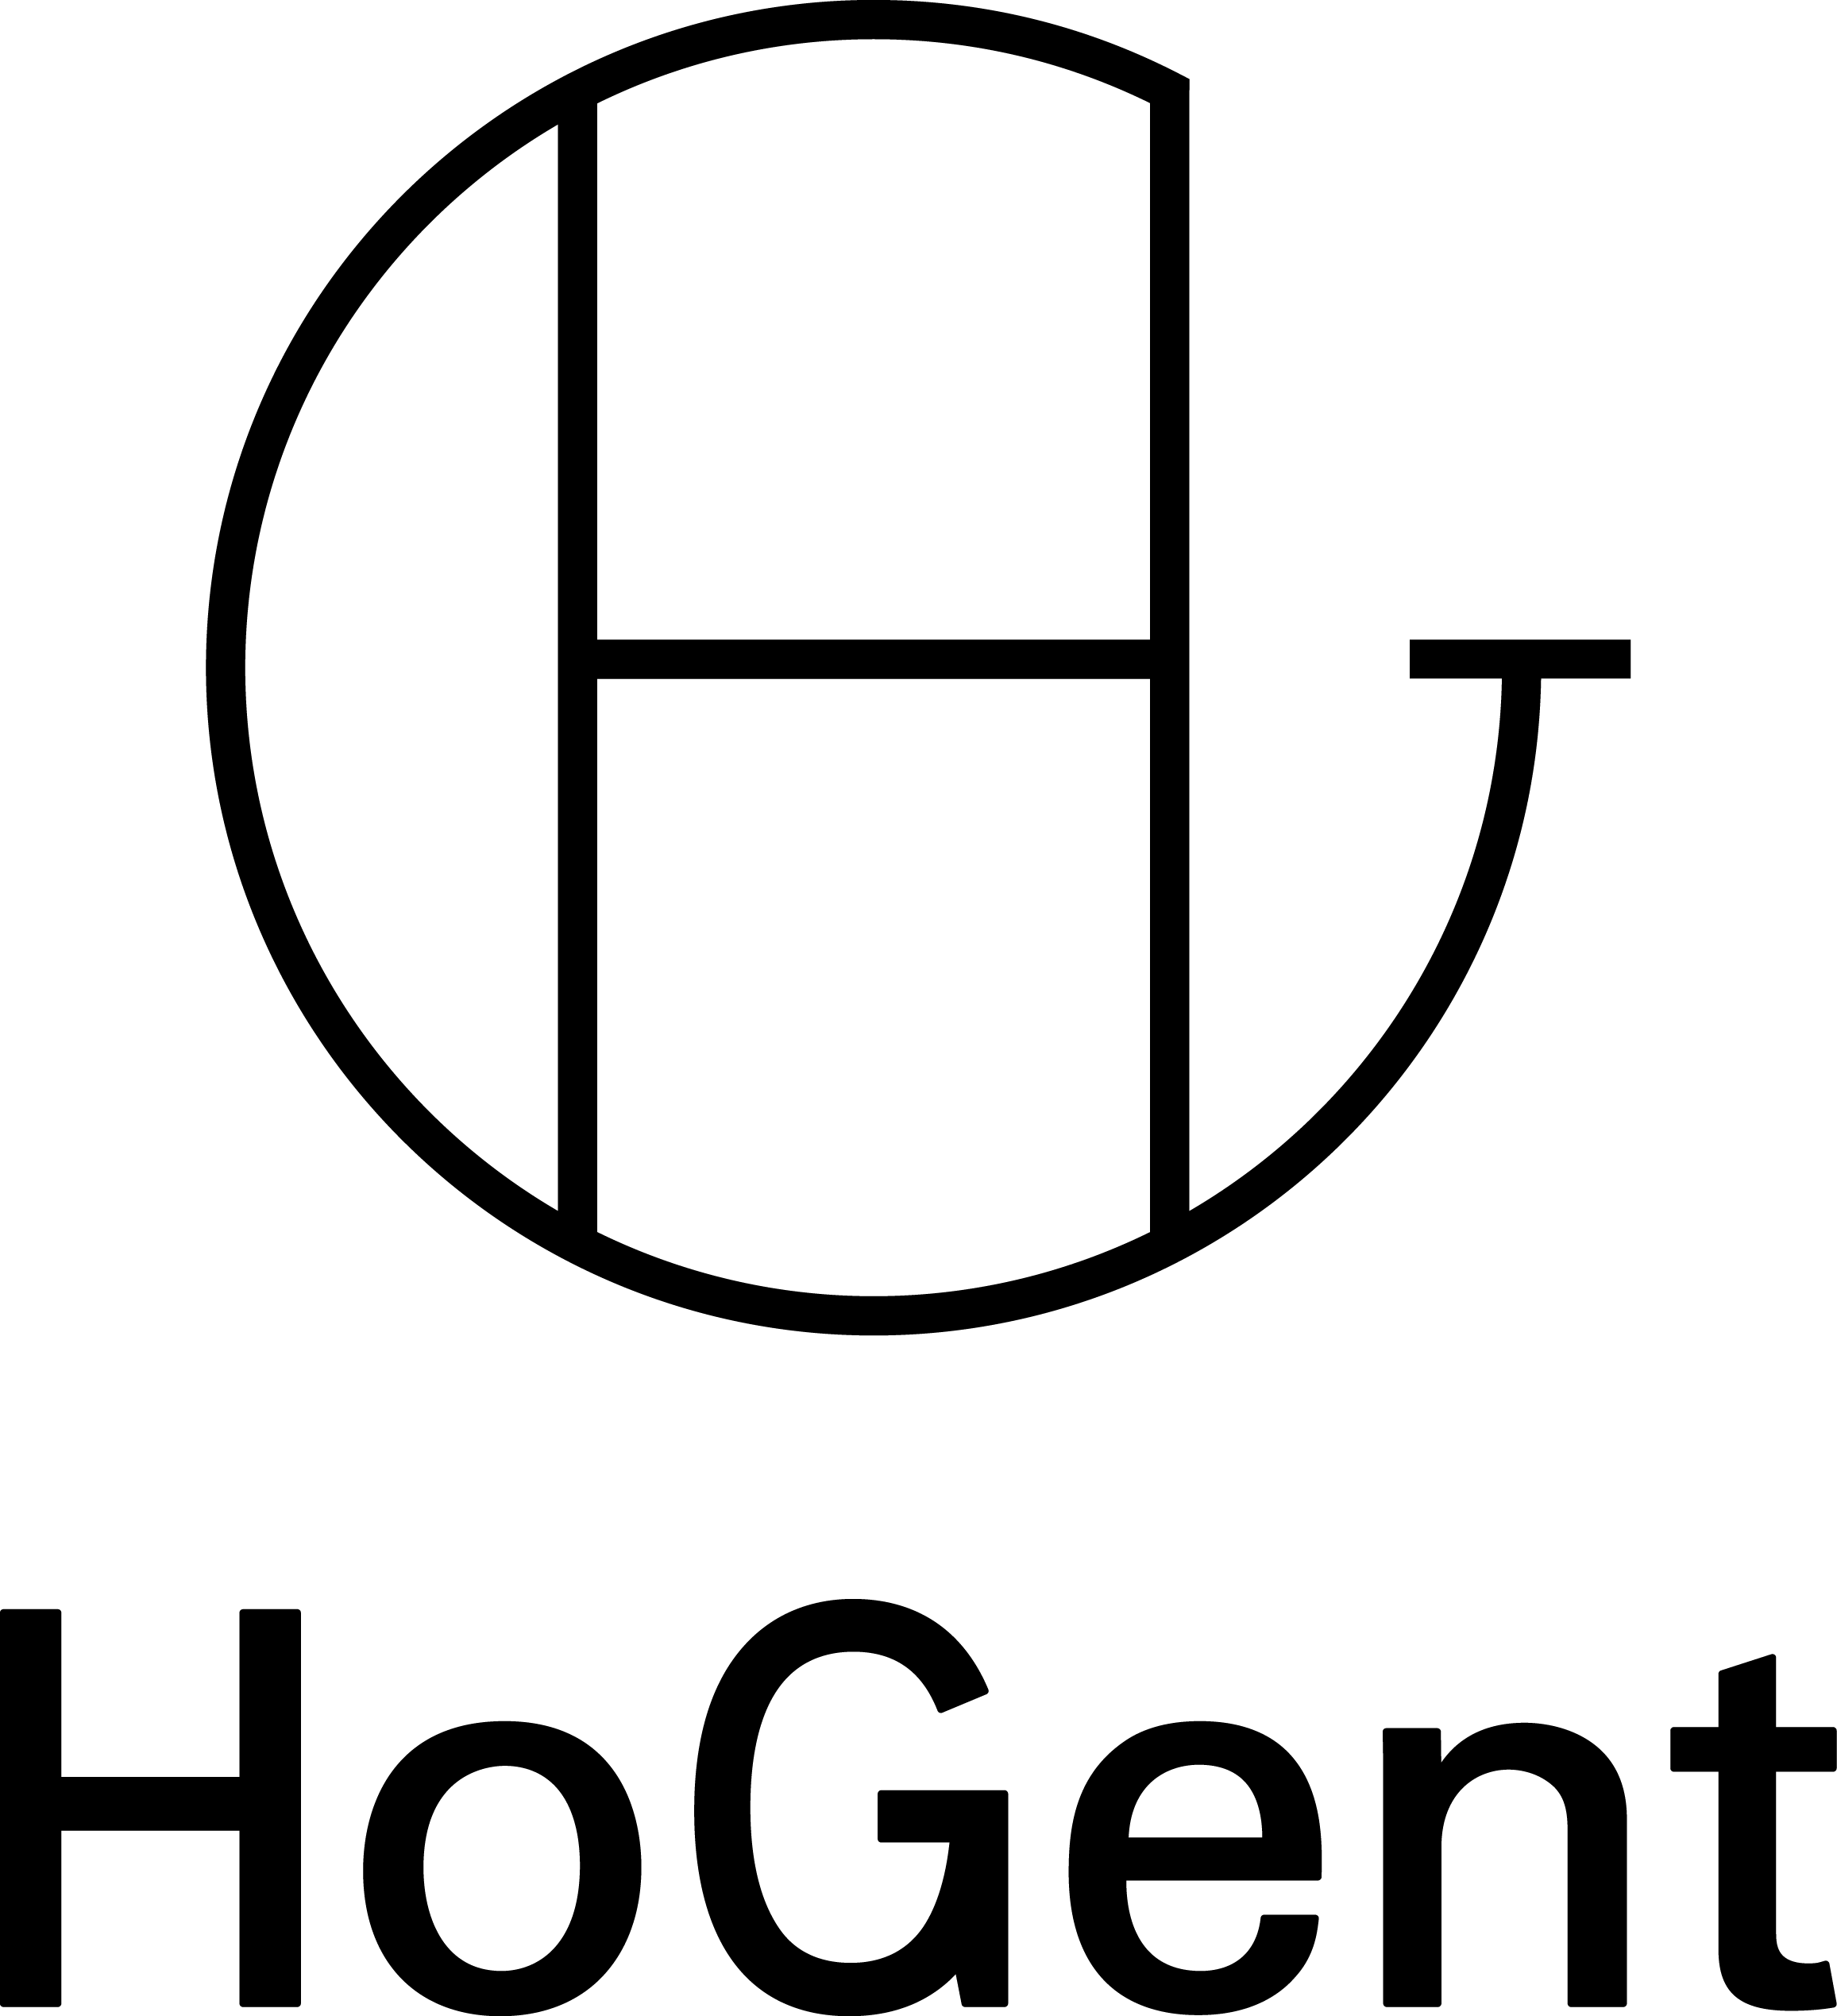
\includegraphics[width=2.5cm]{img/HG-beeldmerk-woordmerk}\\[.5cm]
    Faculteit Bedrijf en Organisatie\\[3cm]
    \titel
    \vfill
    \student\\[3.5cm]
    Scriptie voorgedragen tot het bekomen van de graad van\\professionele bachelor in de toegepaste informatica\\[2cm]
    Promotor:\\
    \promotor\\
    \ifdefempty{\copromotor}{\vspace{2.5cm}}{Co-promotor:\\\copromotor\\[2.5cm]}
    Instelling: \instelling\\[.5cm]
    Academiejaar: \academiejaar\\[.5cm]
    \ifcase \examenperiode \or Eerste \or Tweede \else Derde \fi examenperiode
    \endgroup

  \end{center}
  \restoregeometry
\end{titlepage}
  \emptypage
\begin{titlepage}
  \newgeometry{top=5.35cm,bottom=1.5cm,left=1.5cm,right=1.5cm}
  \begin{center}

    \begingroup
    \rmfamily
    \IfLanguageName{dutch}{Faculteit Bedrijf en Organisatie}{Faculty of Business and Information Management}\\[3cm]
    \titel
    \vfill
    \student\\[3.5cm]
    \IfLanguageName{dutch}{Scriptie voorgedragen tot het bekomen van de graad van\\professionele bachelor in de toegepaste informatica}{Thesis submitted in partial fulfillment of the requirements for the degree of\\professional bachelor of applied computer science}\\[2cm]
    Promotor:\\
    \promotor\\
    \ifdefempty{\copromotor}{\vspace{2.5cm}}{Co-promotor:\\\copromotor\\[2.5cm]}
    \IfLanguageName{dutch}{Instelling}{Institution}: \instelling\\[.5cm]
    \IfLanguageName{dutch}{Academiejaar}{Academic year}: \academiejaar\\[.5cm]
    \IfLanguageName{dutch}{%
    \ifcase \examenperiode \or Eerste \or Tweede \else Derde \fi examenperiode}{%
    \ifcase \examenperiode \or First \or Second \else Third \fi examination period}
    \endgroup

  \end{center}
  \restoregeometry
\end{titlepage}
}

%----------------------------------------------------------------------------------------
%	BIBLIOGRAPHY AND INDEX
%----------------------------------------------------------------------------------------

\usepackage[style=apa,backend=biber]{biblatex}
\usepackage{csquotes}
\DeclareLanguageMapping{dutch}{dutch-apa}
\addbibresource{bachproef-tin.bib} % BibTeX bibliography file
\defbibheading{bibempty}{}

\usepackage{calc} % For simpler calculation - used for spacing the index letter headings correctly
\usepackage{makeidx} % Required to make an index
\makeindex % Tells LaTeX to create the files required for indexing

%----------------------------------------------------------------------------------------
%	MAIN TABLE OF CONTENTS
%----------------------------------------------------------------------------------------

\usepackage{titletoc} % Required for manipulating the table of contents

\contentsmargin{0cm} % Removes the default margin

% Part text styling
\titlecontents{part}[0cm]
{\addvspace{20pt}\centering\large\bfseries}
{}
{}
{}

% Chapter text styling
\titlecontents{chapter}[1.25cm] % Indentation
{\addvspace{12pt}\large\sffamily\bfseries} % Spacing and font options for chapters
{\color{maincolor!60}\contentslabel[\Large\thecontentslabel]{1.25cm}\color{maincolor}} % Chapter number
{\color{maincolor}}
{\color{maincolor!60}\normalsize\;\titlerule*[.5pc]{.}\;\thecontentspage} % Page number

% Section text styling
\titlecontents{section}[1.25cm] % Indentation
{\addvspace{3pt}\sffamily\bfseries} % Spacing and font options for sections
{\contentslabel[\thecontentslabel]{1.25cm}} % Section number
{}
{\hfill\color{black}\thecontentspage} % Page number
[]

% Subsection text styling
\titlecontents{subsection}[1.25cm] % Indentation
{\addvspace{1pt}\sffamily\small} % Spacing and font options for subsections
{\contentslabel[\thecontentslabel]{1.25cm}} % Subsection number
{}
{\ \titlerule*[.5pc]{.}\;\thecontentspage} % Page number
[]

% List of figures
\titlecontents{figure}[0em]
{\addvspace{-5pt}\sffamily}
{\thecontentslabel\hspace*{1em}}
{}
{\ \titlerule*[.5pc]{.}\;\thecontentspage}
[]

% List of tables
\titlecontents{table}[0em]
{\addvspace{-5pt}\sffamily}
{\thecontentslabel\hspace*{1em}}
{}
{\ \titlerule*[.5pc]{.}\;\thecontentspage}
[]

%----------------------------------------------------------------------------------------
%	MINI TABLE OF CONTENTS IN PART HEADS
%----------------------------------------------------------------------------------------

% Chapter text styling
\titlecontents{lchapter}[0em] % Indenting
{\addvspace{15pt}\large\sffamily\bfseries} % Spacing and font options for chapters
{\color{maincolor}\contentslabel[\Large\thecontentslabel]{1.25cm}\color{maincolor}} % Chapter number
{}
{\color{maincolor}\normalsize\sffamily\bfseries\;\titlerule*[.5pc]{.}\;\thecontentspage} % Page number

% Section text styling
\titlecontents{lsection}[0em] % Indenting
{\sffamily\small} % Spacing and font options for sections
{\contentslabel[\thecontentslabel]{1.25cm}} % Section number
{}
{}

% Subsection text styling
\titlecontents{lsubsection}[.5em] % Indentation
{\normalfont\footnotesize\sffamily} % Font settings
{}
{}
{}

%----------------------------------------------------------------------------------------
%	PAGE HEADERS
%----------------------------------------------------------------------------------------

\usepackage{fancyhdr} % Required for header and footer configuration

\pagestyle{fancy}
\renewcommand{\chaptermark}[1]{\markboth{\sffamily\normalsize\bfseries\chaptername\ \thechapter.\ #1}{}} % Chapter text font settings
\renewcommand{\sectionmark}[1]{\markright{\sffamily\normalsize\thesection\hspace{5pt}#1}{}} % Section text font settings
\fancyhf{} \fancyhead[LE,RO]{\sffamily\normalsize\thepage} % Font setting for the page number in the header
\fancyhead[LO]{\rightmark} % Print the nearest section name on the left side of odd pages
\fancyhead[RE]{\leftmark} % Print the current chapter name on the right side of even pages
\renewcommand{\headrulewidth}{0.5pt} % Width of the rule under the header
\addtolength{\headheight}{2.5pt} % Increase the spacing around the header slightly
\renewcommand{\footrulewidth}{0pt} % Removes the rule in the footer
\fancypagestyle{plain}{\fancyhead{}\renewcommand{\headrulewidth}{0pt}} % Style for when a plain pagestyle is specified

% Removes the header from odd empty pages at the end of chapters
\makeatletter
\renewcommand{\cleardoublepage}{
\clearpage\ifodd\c@page\else
\hbox{}
\vspace*{\fill}
\thispagestyle{empty}
\newpage
\fi}

%----------------------------------------------------------------------------------------
%	THEOREM STYLES
%----------------------------------------------------------------------------------------

\usepackage{amsmath,amsfonts,amssymb,amsthm} % For math equations, theorems, symbols, etc

\newcommand{\intoo}[2]{\mathopen{]}#1\,;#2\mathclose{[}}
\newcommand{\ud}{\mathop{\mathrm{{}d}}\mathopen{}}
\newcommand{\intff}[2]{\mathopen{[}#1\,;#2\mathclose{]}}
\newtheorem{notation}{Notation}[chapter]

% Boxed/framed environments
\newtheoremstyle{maincolornumbox}% % Theorem style name
{0pt}% Space above
{0pt}% Space below
{\normalfont}% % Body font
{}% Indent amount
{\small\bf\sffamily\color{maincolor}}% % Theorem head font
{\;}% Punctuation after theorem head
{0.25em}% Space after theorem head
{\small\sffamily\color{maincolor}\thmname{#1}\nobreakspace\thmnumber{\@ifnotempty{#1}{}\@upn{#2}}% Theorem text (e.g. Theorem 2.1)
\thmnote{\nobreakspace\the\thm@notefont\sffamily\bfseries\color{black}---\nobreakspace#3.}} % Optional theorem note
\renewcommand{\qedsymbol}{$\blacksquare$}% Optional qed square

\newtheoremstyle{blacknumex}% Theorem style name
{5pt}% Space above
{5pt}% Space below
{\normalfont}% Body font
{} % Indent amount
{\small\bf\sffamily}% Theorem head font
{\;}% Punctuation after theorem head
{0.25em}% Space after theorem head
{\small\sffamily{\tiny\ensuremath{\blacksquare}}\nobreakspace\thmname{#1}\nobreakspace\thmnumber{\@ifnotempty{#1}{}\@upn{#2}}% Theorem text (e.g. Theorem 2.1)
\thmnote{\nobreakspace\the\thm@notefont\sffamily\bfseries---\nobreakspace#3.}}% Optional theorem note

\newtheoremstyle{blacknumbox} % Theorem style name
{0pt}% Space above
{0pt}% Space below
{\normalfont}% Body font
{}% Indent amount
{\small\bf\sffamily}% Theorem head font
{\;}% Punctuation after theorem head
{0.25em}% Space after theorem head
{\small\sffamily\thmname{#1}\nobreakspace\thmnumber{\@ifnotempty{#1}{}\@upn{#2}}% Theorem text (e.g. Theorem 2.1)
\thmnote{\nobreakspace\the\thm@notefont\sffamily\bfseries---\nobreakspace#3.}}% Optional theorem note

% Non-boxed/non-framed environments
\newtheoremstyle{maincolornum}% % Theorem style name
{5pt}% Space above
{5pt}% Space below
{\normalfont}% % Body font
{}% Indent amount
{\small\bf\sffamily\color{maincolor}}% % Theorem head font
{\;}% Punctuation after theorem head
{0.25em}% Space after theorem head
{\small\sffamily\color{maincolor}\thmname{#1}\nobreakspace\thmnumber{\@ifnotempty{#1}{}\@upn{#2}}% Theorem text (e.g. Theorem 2.1)
\thmnote{\nobreakspace\the\thm@notefont\sffamily\bfseries\color{black}---\nobreakspace#3.}} % Optional theorem note
\renewcommand{\qedsymbol}{$\blacksquare$}% Optional qed square
\makeatother

% Defines the theorem text style for each type of theorem to one of the three styles above
\newcounter{dummy}
\numberwithin{dummy}{section}
\theoremstyle{maincolornumbox}
\newtheorem{theoremeT}[dummy]{Theorem}
\newtheorem{problem}{Problem}[chapter]
\newtheorem{exerciseT}{Exercise}[chapter]
\theoremstyle{blacknumex}
\newtheorem{exampleT}{Example}[chapter]
\theoremstyle{blacknumbox}
\newtheorem{vocabulary}{Vocabulary}[chapter]
\newtheorem{definitionT}{Definition}[section]
\newtheorem{corollaryT}[dummy]{Corollary}
\theoremstyle{maincolornum}
\newtheorem{proposition}[dummy]{Proposition}

%----------------------------------------------------------------------------------------
%	DEFINITION OF COLORED BOXES
%----------------------------------------------------------------------------------------

\RequirePackage[framemethod=default]{mdframed} % Required for creating the theorem, definition, exercise and corollary boxes

% Theorem box
\newmdenv[skipabove=7pt,
skipbelow=7pt,
backgroundcolor=black!5,
linecolor=maincolor,
innerleftmargin=5pt,
innerrightmargin=5pt,
innertopmargin=5pt,
leftmargin=0cm,
rightmargin=0cm,
innerbottommargin=5pt]{tBox}

% Exercise box
\newmdenv[skipabove=7pt,
skipbelow=7pt,
rightline=false,
leftline=true,
topline=false,
bottomline=false,
backgroundcolor=maincolor!10,
linecolor=maincolor,
innerleftmargin=5pt,
innerrightmargin=5pt,
innertopmargin=5pt,
innerbottommargin=5pt,
leftmargin=0cm,
rightmargin=0cm,
linewidth=4pt]{eBox}

% Definition box
\newmdenv[skipabove=7pt,
skipbelow=7pt,
rightline=false,
leftline=true,
topline=false,
bottomline=false,
linecolor=maincolor,
innerleftmargin=5pt,
innerrightmargin=5pt,
innertopmargin=0pt,
leftmargin=0cm,
rightmargin=0cm,
linewidth=4pt,
innerbottommargin=0pt]{dBox}

% Corollary box
\newmdenv[skipabove=7pt,
skipbelow=7pt,
rightline=false,
leftline=true,
topline=false,
bottomline=false,
linecolor=gray,
backgroundcolor=black!5,
innerleftmargin=5pt,
innerrightmargin=5pt,
innertopmargin=5pt,
leftmargin=0cm,
rightmargin=0cm,
linewidth=4pt,
innerbottommargin=5pt]{cBox}

% Creates an environment for each type of theorem and assigns it a theorem text style from the "Theorem Styles" section above and a colored box from above
\newenvironment{theorem}{\begin{tBox}\begin{theoremeT}}{\end{theoremeT}\end{tBox}}
\newenvironment{exercise}{\begin{eBox}\begin{exerciseT}}{\hfill{\color{maincolor}\tiny\ensuremath{\blacksquare}}\end{exerciseT}\end{eBox}}
\newenvironment{definition}{\begin{dBox}\begin{definitionT}}{\end{definitionT}\end{dBox}}
\newenvironment{example}{\begin{exampleT}}{\hfill{\tiny\ensuremath{\blacksquare}}\end{exampleT}}
\newenvironment{corollary}{\begin{cBox}\begin{corollaryT}}{\end{corollaryT}\end{cBox}}

%----------------------------------------------------------------------------------------
%	REMARK ENVIRONMENT
%----------------------------------------------------------------------------------------

\newenvironment{remark}{\par\vspace{10pt}\small % Vertical white space above the remark and smaller font size
\begin{list}{}{
\leftmargin=35pt % Indentation on the left
\rightmargin=25pt}\item\ignorespaces % Indentation on the right
\makebox[-2.5pt]{\begin{tikzpicture}[overlay]
\node[draw=maincolor!60,line width=1pt,circle,fill=maincolor!25,font=\sffamily\bfseries,inner sep=2pt,outer sep=0pt] at (-15pt,0pt){\textcolor{maincolor}{R}};\end{tikzpicture}} % Orange R in a circle
\advance\baselineskip -1pt}{\end{list}\vskip5pt} % Tighter line spacing and white space after remark

%----------------------------------------------------------------------------------------
%	SECTION NUMBERING IN THE MARGIN
%----------------------------------------------------------------------------------------

\makeatletter
\renewcommand{\@seccntformat}[1]{\llap{\textcolor{maincolor}{\csname the#1\endcsname}\hspace{1em}}}
\renewcommand{\section}{\@startsection{section}{1}{\z@}
{-4ex \@plus -1ex \@minus -.4ex}
{1ex \@plus.2ex }
{\normalfont\large\sffamily\bfseries}}
\renewcommand{\subsection}{\@startsection {subsection}{2}{\z@}
{-3ex \@plus -0.1ex \@minus -.4ex}
{0.5ex \@plus.2ex }
{\normalfont\sffamily\bfseries}}
\renewcommand{\subsubsection}{\@startsection {subsubsection}{3}{\z@}
{-2ex \@plus -0.1ex \@minus -.2ex}
{.2ex \@plus.2ex }
{\normalfont\small\sffamily\bfseries}}
\renewcommand\paragraph{\@startsection{paragraph}{4}{\z@}
{-2ex \@plus-.2ex \@minus .2ex}
{.1ex}
{\normalfont\small\sffamily\bfseries}}

%----------------------------------------------------------------------------------------
%	PART HEADINGS
%----------------------------------------------------------------------------------------

% numbered part in the table of contents
\newcommand{\@mypartnumtocformat}[2]{%
\setlength\fboxsep{0pt}%
\noindent\colorbox{maincolor!20}{\strut\parbox[c][.7cm]{\ecart}{\color{maincolor!70}\Large\sffamily\bfseries\centering#1}}\hskip\esp\colorbox{maincolor!40}{\strut\parbox[c][.7cm]{\linewidth-\ecart-\esp}{\Large\sffamily\centering#2}}}%
%%%%%%%%%%%%%%%%%%%%%%%%%%%%%%%%%%
% unnumbered part in the table of contents
\newcommand{\@myparttocformat}[1]{%
\setlength\fboxsep{0pt}%
\noindent\colorbox{maincolor!40}{\strut\parbox[c][.7cm]{\linewidth}{\Large\sffamily\centering#1}}}%
%%%%%%%%%%%%%%%%%%%%%%%%%%%%%%%%%%
\newlength\esp
\setlength\esp{4pt}
\newlength\ecart
\setlength\ecart{1.2cm-\esp}
\newcommand{\thepartimage}{}%
\newcommand{\partimage}[1]{\renewcommand{\thepartimage}{#1}}%
\def\@part[#1]#2{%
\ifnum \c@secnumdepth >-2\relax%
\refstepcounter{part}%
\addcontentsline{toc}{part}{\texorpdfstring{\protect\@mypartnumtocformat{\thepart}{#1}}{\partname~\thepart\ ---\ #1}}
\else%
\addcontentsline{toc}{part}{\texorpdfstring{\protect\@myparttocformat{#1}}{#1}}%
\fi%
\startcontents%
\markboth{}{}%
{\thispagestyle{empty}%
\begin{tikzpicture}[remember picture,overlay]%
\node at (current page.north west){\begin{tikzpicture}[remember picture,overlay]%
\fill[maincolor!20](0cm,0cm) rectangle (\paperwidth,-\paperheight);
\node[anchor=north] at (4cm,-3.25cm){\color{maincolor!40}\fontsize{220}{100}\sffamily\bfseries\@Roman\c@part};
\node[anchor=south east] at (\paperwidth-1cm,-\paperheight+1cm){\parbox[t][][t]{8.5cm}{
\printcontents{l}{0}{\setcounter{tocdepth}{1}}%
}};
\node[anchor=north east] at (\paperwidth-1.5cm,-3.25cm){\parbox[t][][t]{15cm}{\strut\raggedleft\color{white}\fontsize{30}{30}\sffamily\bfseries#2}};
\end{tikzpicture}};
\end{tikzpicture}}%
\@endpart}
\def\@spart#1{%
\startcontents%
\phantomsection
{\thispagestyle{empty}%
\begin{tikzpicture}[remember picture,overlay]%
\node at (current page.north west){\begin{tikzpicture}[remember picture,overlay]%
\fill[maincolor!20](0cm,0cm) rectangle (\paperwidth,-\paperheight);
\node[anchor=north east] at (\paperwidth-1.5cm,-3.25cm){\parbox[t][][t]{15cm}{\strut\raggedleft\color{white}\fontsize{30}{30}\sffamily\bfseries#1}};
\end{tikzpicture}};
\end{tikzpicture}}
\addcontentsline{toc}{part}{\texorpdfstring{%
\setlength\fboxsep{0pt}%
\noindent\protect\colorbox{maincolor!40}{\strut\protect\parbox[c][.7cm]{\linewidth}{\Large\sffamily\protect\centering #1\quad\mbox{}}}}{#1}}%
\@endpart}
\def\@endpart{\vfil\newpage
\if@twoside
\if@openright
\null
\thispagestyle{empty}%
\newpage
\fi
\fi
\if@tempswa
\twocolumn
\fi}

%----------------------------------------------------------------------------------------
%	CHAPTER HEADINGS
%----------------------------------------------------------------------------------------

% A switch to conditionally include a picture, implemented by  Christian Hupfer
\newif\ifusechapterimage
\usechapterimagetrue
\newcommand{\thechapterimage}{}%
\newcommand{\chapterimage}[1]{\ifusechapterimage\renewcommand{\thechapterimage}{#1}\fi}%
\def\@makechapterhead#1{%
{\parindent \z@ \raggedright \normalfont
\ifnum \c@secnumdepth >\m@ne
\if@mainmatter
\begin{tikzpicture}[remember picture,overlay]
\node at (current page.north west)
{\begin{tikzpicture}[remember picture,overlay]
\node[anchor=north west,inner sep=0pt] at (0,0) {\ifusechapterimage\includegraphics[width=\paperwidth]{\thechapterimage}\fi};
\draw[anchor=west] (\Gm@lmargin,-9cm) node [line width=2pt,rounded corners=15pt,draw=maincolor,fill=white,fill opacity=0.5,inner sep=15pt]{\strut\makebox[22cm]{}};
\draw[anchor=west] (\Gm@lmargin+.3cm,-9cm) node {\huge\sffamily\bfseries\color{black}\thechapter. #1\strut};
\end{tikzpicture}};
\end{tikzpicture}
\else
\begin{tikzpicture}[remember picture,overlay]
\node at (current page.north west)
{\begin{tikzpicture}[remember picture,overlay]
\node[anchor=north west,inner sep=0pt] at (0,0) {\ifusechapterimage\includegraphics[width=\paperwidth]{\thechapterimage}\fi};
\draw[anchor=west] (\Gm@lmargin,-9cm) node [line width=2pt,rounded corners=15pt,draw=maincolor,fill=white,fill opacity=0.5,inner sep=15pt]{\strut\makebox[22cm]{}};
\draw[anchor=west] (\Gm@lmargin+.3cm,-9cm) node {\huge\sffamily\bfseries\color{black}#1\strut};
\end{tikzpicture}};
\end{tikzpicture}
\fi\fi\par\vspace*{270\p@}}}

%-------------------------------------------

\def\@makeschapterhead#1{%
\begin{tikzpicture}[remember picture,overlay]
\node at (current page.north west)
{\begin{tikzpicture}[remember picture,overlay]
\node[anchor=north west,inner sep=0pt] at (0,0) {\ifusechapterimage\includegraphics[width=\paperwidth]{\thechapterimage}\fi};
\draw[anchor=west] (\Gm@lmargin,-9cm) node [line width=2pt,rounded corners=15pt,draw=maincolor,fill=white,fill opacity=0.5,inner sep=15pt]{\strut\makebox[22cm]{}};
\draw[anchor=west] (\Gm@lmargin+.3cm,-9cm) node {\huge\sffamily\bfseries\color{black}#1\strut};
\end{tikzpicture}};
\end{tikzpicture}
\par\vspace*{270\p@}}
\makeatother

%----------------------------------------------------------------------------------------
%	HYPERLINKS IN THE DOCUMENTS
%----------------------------------------------------------------------------------------

\usepackage{hyperref}
\hypersetup{hidelinks,backref=true,pagebackref=true,hyperindex=true,colorlinks=false,breaklinks=true,urlcolor= maincolor,bookmarks=true,bookmarksopen=false,pdftitle={Title},pdfauthor={Author}}
\usepackage{bookmark}
\bookmarksetup{
open,
numbered,
addtohook={%
\ifnum\bookmarkget{level}=0 % chapter
\bookmarksetup{bold}%
\fi
\ifnum\bookmarkget{level}=-1 % part
\bookmarksetup{color=maincolor,bold}%
\fi
}
}

%----------------------------------------------------------------------------------------
%	Java source code
%----------------------------------------------------------------------------------------

% Commando voor invoegen Java-broncodebestanden (dank aan Niels Corneille)
% Gebruik:
%   \codefragment{source/MijnKlasse.java}{Uitleg bij de code}
%
% Je kan dit aanpassen aan de taal die je zelf het meeste gebruikt in je
% bachelorproef.
\newcommand{\codefragment}[2]{ \lstset{%
  language=java,
  breaklines=true,
  float=th,
  caption={#2},
  basicstyle=\scriptsize,
  frame=single,
  extendedchars=\true
}
\lstinputlisting{#1}}

% Leeg blad
\newcommand{\emptypage}{%
\newpage
\thispagestyle{empty}
\mbox{}
\newpage
}


%%---------- Documenteigenschappen --------------------------------------------
%% TODO: Vul dit aan met je eigen info:

% Je eigen naam
\newcommand{\student}{Robin Malfait}

% De naam van je promotor (lector van de opleiding)
\newcommand{\promotor}{Lieven Smits}

% De naam van je co-promotor. Als je promotor ook je opdrachtgever is en je
% dus ook inhoudelijk begeleidt (en enkel dan!), mag je dit leeg laten.
\newcommand{\copromotor}{Mathias Verraes}

% Indien je bachelorproef in opdracht van/in samenwerking met een bedrijf of
% externe organisatie geschreven is, geef je hier de naam. Zoniet laat je dit
% zoals het is.
\newcommand{\instelling}{---}

% De titel van het rapport/bachelorproef
\newcommand{\titel}{Wanneer is EventSourcing een meerwaarde voor een bedrijf zoals Skedify, waar ze gespecialiseerd zijn in online scheduling?}

% Datum van indienen (gebruik telkens de deadline, ook al geef je eerder af)
\newcommand{\datum}{02 juni 2017}

% Academiejaar
\newcommand{\academiejaar}{2016-2017}

% Examenperiode
%  - 1e semester = 1e examenperiode => 1
%  - 2e semester = 2e examenperiode => 2
%  - tweede zit  = 3e examenperiode => 3
\newcommand{\examenperiode}{2}

%%=============================================================================
%% Inhoud document
%%=============================================================================

\begin{document}

%---------- Taalselectie ------------------------------------------------------
%% Als je je bachelorproef in het Engels schrijft, haal dan onderstaande regel
%% uit commentaar. Let op: de tekst op de voorkaft blijft in het Nederlands, en
%% dat is ook de bedoeling!
%\selectlanguage{english}

%---------- Titelblad ---------------------------------------------------------
\inserttitlepage

%---------- Samenvatting, voorwoord -------------------------------------------
\usechapterimagefalse
%%=============================================================================
%% Samenvatting
%%=============================================================================

%% TODO: De "abstract" of samenvatting is een kernachtige (~ 1 blz. voor een
%% thesis) synthese van het document.
%%
%% Deze aspecten moeten zeker aan bod komen:
%% - Context: waarom is dit werk belangrijk?
%% - Nood: waarom moest dit onderzocht worden?
%% - Taak: wat heb je precies gedaan?
%% - Object: wat staat in dit document geschreven?
%% - Resultaat: wat was het resultaat?
%% - Conclusie: wat is/zijn de belangrijkste conclusie(s)?
%% - Perspectief: blijven er nog vragen open die in de toekomst nog kunnen
%%    onderzocht worden? Wat is een mogelijk vervolg voor jouw onderzoek?
%%
%% LET OP! Een samenvatting is GEEN voorwoord!

%%---------- Samenvatting -----------------------------------------------------
%%
%% De samenvatting in de hoofdtaal van het document

\chapter*{\IfLanguageName{dutch}{Samenvatting}{Abstract}}

%% Context: waarom is dit werk belangrijk
Deze maatschappij draait om data. Data en informatie zijn geld waard, daarom is het van belang dat er voorzichtig mee om wordt gegaan. In systemen waar relationele modellen gebruikt worden gaat er data verloren. Telkens wanneer er een UPDATE of DELETE sql statement wordt uitgevoerd is deze informatie er niet meer. Door middel van EventSourcing gaat er geen data verloren.
%% - Nood: waarom moest dit onderzocht worden?
Het is van belang om informatie bij te houden, dit kan altijd interessant zijn in de toekomst wanneer er specifieke business vragen komen waar er momenteel nog geen antwoord op is.
%% - Taak: wat heb je precies gedaan?
%% - Object: wat staat in dit document geschreven?
Eerst wordt er gegekeken naar al de delen die deel uitmaken van een EventSourced applicatie. Dit gaat van CQS, CQRS tot de effectieve onderdelen van EventSourcing. Er wordt ook uitleg gegeven over Skedify zodat de concrete businesscase duidelijk gescoped wordt.
%% - Resultaat: wat was het resultaat?
%% - Conclusie: wat is/zijn de belangrijkste conclusie(s)?
%% - Perspectief: blijven er nog vragen open die in de toekomst nog kunnen
%%    onderzocht worden? Wat is een mogelijk vervolg voor jouw onderzoek?
%%=============================================================================
%% Voorwoord
%%=============================================================================

\chapter*{Voorwoord}
\label{ch:voorwoord}

%% TODO:
%% Het voorwoord is het enige deel van de bachelorproef waar je vanuit je
%% eigen standpunt (``ik-vorm'') mag schrijven. Je kan hier bv. motiveren
%% waarom jij het onderwerp wil bespreken.
%% Vergeet ook niet te bedanken wie je geholpen/gesteund/... heeft

Ik ben al een 5 jaar lang gepassioneerd door data en informatie. Door gebruik te maken van EventSourcing gaat er geen informatie verloren, en is er een mogelijkheid om te tijdreizen. Het is mogelijk om een rapport te schrijven in het heden, terug te gaan naar het begin der tijden van de applicatie en daar het rapport te genereren alsof het rapport toen al bestond. Het idee van deze bachelorproef kwam voort uit gesprekken met een aantal mensen via de sociale media Twitter. Deze mensen zijn nu bekend in de \gls{DDD} en EventSourcing wereld. Een van deze mensen is Shawn McCool, die het platform https://eventsourcery.com heeft gemaakt, wat een introductie is tot domain modeling, \gls{CQRS} (zie Hoofdstuk~\ref{ch:CQRS}) en EventSourcing (zie Hoofdstuk~\ref{ch:eventsourcing}).

Dankzij Twitter heb ik ook mijn co-promotor, Mathias Verraes, leren kennen. Ik heb hem ook ontmoet op een conferentie in Nederland, namelijk Laracon EU 2014. Ik zou hem heel graag willen bedanken voor het helpen realiseren van deze bachelorproef. Ik kon altijd met al mijn vragen terecht bij hem, en hij bezorgde mij ook de nodige boeken, blog posts en andere resources omtrent EventSourcing. Ik kreeg ook de kans om naar \gls{meetup}\footnote{\glsdesc{meetup}} te gaan, maar dit was niet altijd even gemakkelijk omdat ze niet altijd bij de deur plaatsvonden.

Ik zou ook graag de product owner van Skedify, Christophe Thelen, bedanken om mij interessante gegevens over Skedify te bezorgen, alsook resources in verband met EventSourcing omdat hij hier ook al in de praktijk mee gewerkt heeft.

Daarnaast zou ik ook graag mijn promotor, Lieven Smits, willen bedanken voor het benadrukken van mijn spellingsfouten, mij te helpen bij het herstructureren van bepaalde delen en in het algemeen om deze bachelorproef tot een goed einde te brengen.

Tot slot zou ik ook graag mijn vriendin willen bedanken voor het extra nalezen van mijn bachelorproef en mij te steunen in deze drukke tijden.

%---------- Inhoudstafel ------------------------------------------------------
\pagestyle{empty} % No headers
\tableofcontents % Print the table of contents itself
\cleardoublepage % Forces the first chapter to start on an odd page so it's on the right
\pagestyle{fancy} % Print headers again

%---------- Lijst afkortingen, termen -----------------------------------------
%% Als je een lijst van afkortingen of termen wil toevoegen, dan hoort die
%% hier thuis. Gebruik bijvoorbeeld de ``glossaries'' package.

%%---------- Kern -------------------------------------------------------------

%%=============================================================================
%% Inleiding
%%=============================================================================

\chapter{Inleiding}
\label{ch:inleiding}

De inleiding moet de lezer alle nodige informatie verschaffen om het onderwerp te begrijpen zonder nog externe werken te moeten raadplegen \autocite{Pollefliet2011}. Dit is een doorlopende tekst die gebaseerd is op al wat je over het onderwerp gelezen hebt (literatuuronderzoek).

Je verwijst bij elke bewering die je doet, vakterm die je introduceert, enz. naar je bronnen. In \LaTeX{} kan dat met het commando \texttt{$\backslash${textcite\{\}}} of \texttt{$\backslash${autocite\{\}}}. Als argument van het commando geef je de ``sleutel'' van een ``record'' in een bibliografische databank in het Bib\TeX{}-formaat (een tekstbestand). Als je expliciet naar de auteur verwijst in de zin, gebruik je \texttt{$\backslash${}textcite\{\}}.
Soms wil je de auteur niet expliciet vernoemen, dan gebruik je \texttt{$\backslash${}autocite\{\}}. Hieronder een voorbeeld van elk.

\textcite{Knuth1998} schreef een van de standaardwerken over sorteer- en zoekalgoritmen. Experten zijn het erover eens dat cloud computing een interessante opportuniteit vormen, zowel voor gebruikers als voor dienstverleners op vlak van informatietechnologie~\autocite{Creeger2009}.

\section{Stand van zaken}
\label{sec:stand-van-zaken}

%% TODO: deze sectie (die je kan opsplitsen in verschillende secties) bevat je
%% literatuurstudie. Vergeet niet telkens je bronnen te vermelden!

\section{Probleemstelling en Onderzoeksvragen}
\label{sec:onderzoeksvragen}

%% Uit je probleemstelling moet duidelijk zijn dat je onderzoek een meerwaarde
%% heeft voor een concrete doelgroep (bv. een bedrijf).
%%
%% Wees zo concreet mogelijk bij het formuleren van je
%% onderzoeksvra(a)g(en). Een onderzoeksvraag is trouwens iets waar nog
%% niemand op dit moment een antwoord heeft (voor zover je kan nagaan).
Data is belangrijk, rapportering is belangrijk. Voorspellen van vragen die de business kan vragen binnen dit en 5 jaar is onmogelijk. Daarom is het heel belangrijk om alle informatie bij te houden om hier interessante rapportering op te kunnen uitvoeren. In een systeem met een standaard relationele databank wordt niet alle informatie bijgehouden. Bij het verwijderen of wijzigen van informatie is de voorgaande informatie verloreren gegaan. Alle informatie bijhouden is dus interessant, maar wat zijn hier de voor en nadelen van?

De onderzoeksvraag luidt als volgt: Wanneer is EventSourcing een meerwaarde voor een bedrijf zoals Skedify, waar ze gespecialiseerd zijn in online scheduling?

Hierbij worden ook volgende subvragen beantwoord:

\begin{itemize}
    \item Wat is het verschil tussen een systeem met relationele databank modellen en een systeem met EventSourcing?
    \item Hoe kan een applicatie die gebruik maakt van EventSourcing getest worden?
    \item Welke delen moeten er EventSourced worden, en hoe kan je deze delen bepalen?
\end{itemize}

\section{Opzet van deze bachelorproef}
\label{sec:opzet-bachelorproef}

%% TODO: Het is gebruikelijk aan het einde van de inleiding een overzicht te
%% geven van de opbouw van de rest van de tekst. Deze sectie bevat al een aanzet
%% die je kan aanvullen/aanpassen in functie van je eigen tekst.

De rest van deze bachelorproef is als volgt opgebouwd:

In Hoofdstuk~\ref{ch:methodologie} wordt de methodologie toegelicht en worden de gebruikte onderzoekstechnieken besproken om een antwoord te kunnen formuleren op de onderzoeksvragen.

%% TODO: Vul hier aan voor je eigen hoofstukken, één of twee zinnen per hoofdstuk

In Hoofdstuk~\ref{ch:conclusie}, tenslotte, wordt de conclusie gegeven en een antwoord geformuleerd op de onderzoeksvragen. Daarbij wordt ook een aanzet gegeven voor toekomstig onderzoek binnen dit domein.


%%=============================================================================
%% Methodologie
%%=============================================================================

\chapter{Methodologie}
\label{ch:methodologie}

%% TODO: Hoe ben je te werk gegaan? Verdeel je onderzoek in grote fasen, en
%% licht in elke fase toe welke stappen je gevolgd hebt. Verantwoord waarom je
%% op deze manier te werk gegaan bent. Je moet kunnen aantonen dat je de best
%% mogelijke manier toegepast hebt om een antwoord te vinden op de
%% onderzoeksvraag.


Voor er een proof of concept gemaakt kan worden in verband met EventSourcing, moet er eerst gekeken worden naar wat EventSourcing is en wat het inhoudt. Naast EventSourcing zijn er ook concepten zoals CQRS die aan bod moeten komen. Daarnaast draait het in dit onderzoek rond Skedify, het bedrijf die als concrete case gebruikt zal worden. In het deel rond Skedify, kan er meer te weten gekomen worden in verband met wat ze doen en hoe ze te werk gaan. Daarna zal er gekeken worden naar de huidige manier van werken. Tot slot gaat alles worden samengevoegd: Skedify en de huidige manier van werken, en Skedify en EventSourcing. Hierna worden de voor- en nadelen van beide mogelijkheden afgaan om te zien of EventSourcing nu effectief een meerwaarde biedt voor Skedify. Het onderzoek is in grote delen opgesplitst: Skedify, EventSourcing, huidige manier van werken en de conclusies.

In het deel over Skedify zal er onderzocht worden wat ze doen, en hoe ze dit doen. Er zal ook een gesprek komen met de business kant van Skedify om vragen te kunnen beantwoorden en om duidelijke conclusies te kunnen trekken.

In het deel over EventSourcing zal er dieper onderzocht worden hoe EventSourcing juist werkt en hoe het gebruikt kan worden.
\section{Literatuurstudie}
\label{sec:literatuurstudie}

...TODO...
\section{Proof of concept}
\label{sec:proof-of-concept}

Voor de proof-of-concept zullen bepaalde functies van Skedify geschreven worden in het huidige systeem en in een EventSourcing systeem. Daarbij zal er gekeken worden naar voordelen en nadelen van beide systemen.

%% Voeg hier je eigen hoofdstukken toe die de ``corpus'' van je bachelorproef
%% vormen. De structuur en titels hangen af van je eigen onderzoek. Je kan bv.
%% elke fase in je onderzoek in een apart hoofdstuk bespreken.

%%=============================================================================
%% Skedify
%%=============================================================================

\chapter{Skedify}
\label{ch:skedify}

Skedify is een Gentse tech start-up dat online afspraakbeheersoftware ontwikkelt voor onder andere de banksector, ziekenfondsen, verzekeringen, immobiliën en HR-bedrijven. Deze bachelorproef gaat op zoek naar een antwoord of EventSourcing een meerwaarde kan bieden voor Skedify. Skedify zorgt er voor dat een persoon in eender welke sector een afspraak kan maken op een korte tijd voor eender welk probleem, en dit met de juiste contactpersoon van het bedrijf. Dit moet in een zo kort mogelijke tijd verlopen. Skedify is een business-to-business tool, die onder andere dynamisch formulieren kan gaan opbouwen om te gebruiken in de plugin die op de website van de klant terecht komt. Alle informatie binnen het systeem wordt in een relationele databank opgeslagen.

Een van de mogelijkheden die Skedify biedt is het wijzigen van een afspraak. Het kan interessant zijn om te weten hoeveel keer dit gebeurt en of er specifieke maatregelen kunnen genomen worden.

Rapportering is tot op de dag van vandaag nog niet beschikbaar omdat er geen historiek wordt bijgehouden.
%%=============================================================================
%% CQRS
%%=============================================================================

\chapter{CQRS}
\label{ch:CQRS}

CQRS is een term uitgevonden door Greg Young, de heer Young gaat ook verder in op EventSourcing. Een goede uitleg hieromtrent is te vinden in een presentatie die hij gaf op een conferentie \autocite{Young2014CQRSandES}. CQS kort voor Command Query Seperation, is een principe die uitgevonden is door Bertrand Meyer \autocite{Meyer1988}. Het is een API design principe dat beschrijft hoe er met een object of een systeem gecommuniceerd moet worden. CQRS daarentegen is een architectuurstijl die gaat over hoe het aan de binnenkant geïmplementeerd is. Als er gekeken wordt naar CQS is dit al een eerste vorm van goede, overzichtelijke code schrijven. CQS zorgt er voor dat getters en setters gescheiden zijn. Getters zijn strict bedoeld om een waarde uit de huidige state te halen en deze terug te geven. Setters zijn bedoeld om een wijziging te doen (of een algemene actie uit te voeren), setters geven geen waarde terug maar void, dit principe wordt ook uitegelegd op de blog van Martin Fowler \autocite{Fowler2005CQS}. Een goede heuristiek voor het toepassen van CQS is: "Een vraag stellen, mag het antwoord niet wijzigen.", met andere woorden, een getter heeft nooit gevolgen op de huidige state of op andere zaken.

Het doel van CQS is vooral de leesbaarheid verhogen, het is een principe die developers gebruiken en begrijpen waardoor communicatie makkelijker gaat.
Een tweede probleem is dat getters en setters in een en dezelfde klasse gedefinieerd zijn, voor eenvoudige klassen is dit geen probleem, maar wanneer er gelezen of geschreven wordt naar een databank is dit wel een probleem.. Er is geen stricte scheiding tussen de lees kant en de schrijf kant.

\codefragment{source/CQS-Appointment.java}{Voorbeeld van CQS}

In dit voorbeeld zijn getters en setters strict gescheiden. Het opvragen van een datum of subject wijzigt niets aan de huidige state van dat object. Wanneer deze klasse ook verbonden is aan een databank, dan komen de problemen naar boven.

\codefragment{source/CQS-Appointment-db.java}{Voorbeeld van CQS met databank}

Er is nu geen manier om de lees- en schrijfkant los te koppelen van elkaar.

Dit is waar CQRS komt kijken, Command Query Responsibility Segregation. CQRS zorgt er voor dat de lees- en schrijfkant kant strict gescheiden zijn. Het zijn bijna 2 applicaties die naast elkaar staan. Een Command wordt afgehandeld aan de schrijfkant en een Query wordt afgehandeld aan de leeskant. Zowel een Command als een Query zijn messages, dit wordt verder besproken in hoofdstuk~\ref{sec:messages}. De leeskant gaat zijn informatie halen bij de databank (of een andere vorm van opslagmechanisme), dit kan via sql queries, ORM tools, enzovoort. De manier waarop dit gebeurt staat volledig los van hoe de schrijfkant communiceert met het opslagmechanisme. 

De meeste applicaties, onder andere ook die van Skedify zijn intensiever aan de leeskant dan aan de schrijfkant (Tabel \ref{cqrs-read-writes}). De lees- en schrijfkant zijn nu strict gescheiden en er kan gebruik gemaakt worden van schalingsmechanismen. Beter nog, de leeskant en schrijfkant kunnen individueel geschaald worden. Er kan zelfs geopteerd worden om lees- en schrijfkant in verschillende programmeertalen te schrijven.

\begin{table}[h]
\centering
\caption{Aantal requests vergeleken voor de lees- en schrijfkant. Er zijn ~5.548 (\textasciitilde18.02\%) keer zoveel lees requests dan schrijf requests.}
\begin{tabular}{lll} \toprule
Methode & \# Requests & Type        \\ \midrule
GET     & 612 000     & LEZEN       \\
OPTIONS & 148 000     & LEZEN       \\
POST    & 129 000     & SCHRIJVEN   \\
HEAD    & 362 000     & LEZEN       \\
PATCH   & 13 400      & SCHRIJVEN   \\
DELETE  & 1 100       & SCHRIJVEN   \\ \bottomrule
\end{tabular}
\label{cqrs-read-writes}
\end{table}

\begin{figure}[h]
\caption{Visuele representatie van tabel ~\ref{cqrs-read-writes}}
\centering
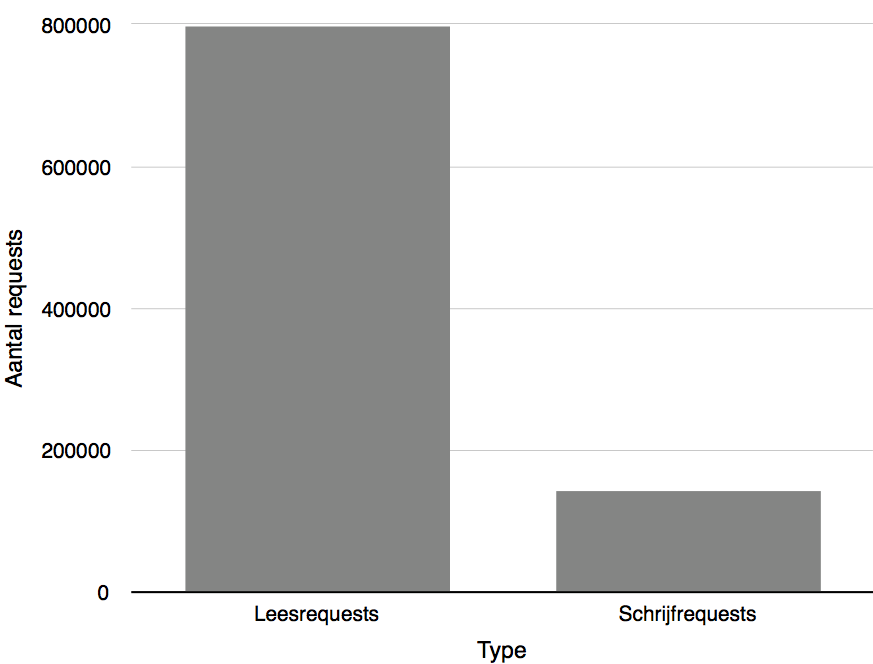
\includegraphics[width=0.75\textwidth]{img/lees-en-schrijfkant}
\end{figure}

Door de zwaardere druk langst de leeskant, kan er moeilijk geoptimaliseerd worden voor alle cases waar zowel de lees- als schrijfkant voordeel uit haalt. De splitsing is daarom een voordeel om langs bijde kanten te kunnen optimaliseren.

Wanneer de lees- en schrijfkant niet gescheiden zouden worden, dan maken ze gebruik van de dezelfde databank. Wanneer er gelezen wordt en door een andere partij geschreven wordt, kan dit elkaar hinderen omdat beide kanten dezelfde resources gebruiken.

CQRS speelt en grote rol bij EventSourcing, vandaar dit korte hoofdstuk.

%%=============================================================================
%% EventSourcing
%%=============================================================================

\chapter{EventSourcing}
\label{ch:eventsourcing}

EventSourcing is geen nieuwe uitvinding, maar wordt al jaren gebruikt in andere sectoren. Bekende voorbeelden zijn de bankindustrie, wetgeving, en patiënten fisches die opgeslagen zijn bij dokters.

EventSourcing, is zoals de naam al verklapt, dat events de bron zijn van de applicatie. Het is ook zo dat de events de "single source of truth" zijn van de applicatie om andere state uit af te leiden. Een log bestaat ook uit een geschiedenis van events, maar deze wordt niet gebruikt als "single source of truth" op de huidige state af te leiden.

Als er naar de bankindustrie wordt gekeken dan is het bedrag op iemand zijn rekening niet een getal dat opgeslagen is in een databank, of toch niet de enige vorm hier van. Er is een lijst van transacties die tot dit getal komen. Het zal ook wel in een databank opgeslagen zijn, maar dit is den puur een caching mechanisme.

Het is zo dat nu pas, de laatste jaren, EventSourcing opkomt in de informatica sector. In de volgende hoofdstukken zal er dieper ingegaan worden op onderdelen van EventSourcing.
  %%=============================================================================
%% Aggregates
%%=============================================================================

\section{Aggregates}
\label{sec:aggregates}

Aggregaten zijn de entiteiten die behoren tot het domein. Een aggregaat is een entiteit die zal zorgen dat invariants (besproken in \ref{sec:invariants}) gegarandeerd zullen worden. Eens dit het geval is zal die er voor zorgen dat de juiste domain events opgeslagen worden en de state van de applicatie wordt gewijzigd.

Deze aggregaten moeten correct gekozen worden, zodat er geen gevaar is dat er 'god' aggregaten ontstaan. Een 'god' aggregaat is een aggregaat die alles in een applicatie doet, in de meeste gevallen is dit een 'User' aggregaat.

In het geval van Skedify zijn goede aggregaten: Appointment, Subject, Question, Answer, Office, ...
  %%=============================================================================
%% Value Objects
%%=============================================================================

\section{Value Objects}
\label{sec:value-objects}

Value objects zijn objecten die zorgen dat een bepaalde waarde altijd in een geldige staat is. Bijvoorbeeld, er kan een value object zijn voor een Email. Dit email adres moet ten alle tijden geldig zijn. Dit kan afgedwongen worden door in de constructor van een klasse een waarde te ontvangen en deze te controleren. Indien deze waarde fout is wordt er een exceptie gegooid. Deze exceptie zal dan opgevangen worden in de lagen daarboven.

Een belangrijke regel bij Value objects is dat deze geen identiteit bevatten, ze hebben geen unieke identifier en zijn daarom geen entiteit. Value objects kunnen wel tot een entiteit behoren zoals Bijvoorbeeld een User entiteit.

  %%=============================================================================
%% Messages
%%=============================================================================

\section{Messages}
\label{sec:messages}

Communicatie in een applicatie draait rond messages. Er zijn 3 soorten messages die terug komen in een applicatie: informational, interrogatory en imperative. \textcite{Verraes2015Messages}
Binnen een applicatie met EventSourcing wordt er ook gebruik gemaakt van messages.


\subsection{Imperative Messages}
\label{subsec:imperative-messages}

De imperative of imperatieve messages, zijn messages die de intentie hebben om de ontvanger van dit bericht een actie te laten uitvoeren.
Binnen EventSourcing zijn is een typisch voorbeeld een Command, waarbij het Command de intentie heeft om een actie uit te voeren. Binnen een systeem zijn deze Commands iets typisch dat uit de business kant komt. Wanneer het volgende voorbeeld door iemand van de business gelezen wordt, weet die ook meteen wat er zal gebeuren, als er gewerkt wordt met deze Command.

\codefragment{source/Messages-ChangeAppointmentStartDate.java}{Een voorbeeld van een Command}

Wanneer er met deze klasse gewerkt wordt (of met objecten van deze klasse), dan wordt er verwacht dat de ontvanger iets zal wijzigen.

\subsection{Interrogatory Messages}
\label{subsec:interrogatory-messages}

De interrogatory of ondervragende messages, zijn messages die iets vragen over de huidige state van de applicatie. In elke applicatie worden er zaken opgevraagd. Binnen EventSourcing wordt dit ook gedaan aan de hand van Queries, deze Queries gaan informatie opvragen van de huidige state. Deze queries worden ook opgelegd door de business kant, de business kan, wanneer ze het voorbeeld zien, meteen begrijpen wat er zal gebeuren als er met deze Query wordt gewerkt.

\codefragment{source/Messages-MyAppointmentsForToday.java}{Een voorbeeld van een Query}

Bij dit voorbeeld is het duidelijk det er informatie opgevraagd wordt en dat er geen wijzigingen aan de huidige state zullen gebeuren.

\subsection{Informational Messages}
\label{subsec:informational-messages}

De informational of de informatieve messages, zijn messages die iets over zichzelf willen vertellen. Bij EventSourcing wordt dit uitgedrukt in DomainEvents. DomainEvents zijn de messages die opgeslagen zullen worden in de databank. DomainEvents worden ook meestal in de verleden tijd geschreven omdat ze benadrukken dat er iets gebeurt is.

\codefragment{source/Messages-AppointmentsStartDateHasBeenChanged.java}{Een voorbeeld van een DomainEvent}

Dit voorbeeld lijkt sterk om het voorbeeld van de Command, maar de intentie van beide klassen is totaal verschillend. De klasnamen zijn altijd expliciet, soms zijn ze wat lang maar het is duidelijk wat de bedoeling is. Doordat de messages zo expliciet geschreven zijn, kan er gemakkelijk mee gecommuniceerd worden wat het hele doel is van messages.

Er mag ook geen gemeenschappelijke naam gezocht worden voor deze klassen om 'dubbele code' te verwijderen. Vanaf dit gebeurt komen er problemen naar boven. Wat als er extra informatie in een Command moet maar niet in een DomainEvent of vice versa. De leesbaarheid van de code gaat ook achteruit, de communicatie wordt onduidelijk.

  %%=============================================================================
%% Domain Events
%%=============================================================================

\section{Domain Events}
\label{sec:domain-events}

Domain events zijn een relevant onderdeel van EventSourcing. Domain Events zijn, net als commands and queries, messages. Domain Events zijn de effectieve events die zullen opgeslagen worden in een append-only database. Een event is iets dat gebeurt is en nooit meer kan veranderen. Er zijn een paar belangrijke eigenschappen aan deze events.

\begin{itemize}
  \item{Ze bevatten een unieke id, die op voorhand vastgelegd is. Dit kan een GUID (Globally Unique Identifier) zijn.}
  \item{Ze bevatten enkel de data die gewijzigd is ten opzichte van de vorige versie.}
  \item{Alle data die ze bevatten, is correct en kan niet meer aangepast worden.}
\end{itemize}

Domain events worden opgeslagen in een append-only database, maar wat als er een fout gemaakt is gemaakt?
Indien een fout is opgetreden, moet er een nieuw domain event gemaakt worden, die het vorige event corrigeerd. Op deze manier blijft al de data correct, en gaat er geen belangrijke informatie verloren. Er is ook niet geprutst met de historiek van deze events, wat van belang is omdat de geschiedenis herschrijven gevolgen kan hebben voor een systeem. Het houdt in dat de audit log (hoofdstuk~\ref{sec:audit-log}) niet meer geldig is. Het houdt ook in dat elke projectie opnieuw zal moeten opgebouwd, omdat een wijziging in 1 event een totaal andere uitkomst kan creëren in de huidige state.

Domain events hebben ook een naam, deze naam is specifiek voor de use case. Het verteld meer over wat er gebeurt is of wat er zal gebeuren. Het is ook aangeraden dat deze naam in de verleden tijd is opgesteld. Zo kan er gedifferentieerd worden tussen de soorten messages (hoofdstuk~\ref{sec:messages}) en kan de leesbaarheid verhoogd worden naar andere partijen toe (developers, business). Een event is tenslotte gebeurd. Als er in context van Skedify gesproken wordt, dan is AppointmentWasRescheduled een goede naam voor een domain event. Het is ook van belang dat er geen CRUD (Create Read Update Delete) events gemaakt worden zoals OfficeWasCreated, want er werd niet effectief een office gemaakt, er is een office toegevoegd. Een betere naam zou zijn OfficeWasAdded.

  %%=============================================================================
%% Invariants
%%=============================================================================

\section{Invariants}
\label{sec:invariants}

Invariants zijn regels die opgelegd zijn door de business. Invariants worden gecontroleerd alvorens een domain event opgeslagen wordt. Elke invariant moet goedgekeurd, want eens een domain event opgeslagen is, kan dit niet meer ongedaan gemaakt worden. Er kan wel een nieuw domain event opgeslagen worden om deze wijziging te niet te doen. Invariant controle wordt uitgevoerd, en telkens wanneer een input niet aan deze invariant voldoet moet er een exception gegooid worden.


  %%=============================================================================
%% Eventual Consistency
%%=============================================================================

\section{Eventual Consistency}
\label{sec:eventual-consistency}

...TODO...
  %%=============================================================================
%% Event Store
%%=============================================================================

\section{Event Store}
\label{sec:event-store}

De EventStore is een relevant concept bij EventSourcing. De EventStore is de plaats waar alle DomainEvents opgeslagen zullen worden. De EventStore kan elk soort databank zijn, er is ook een speciaal gemaakt en is te vinden op https://geteventstore.com. Voor deze bachelorproef, en de proof-of-concept zal er gebruik gemaakt worden van een simpele EventStore in mysql. Een EventStore is helemaal niet zo moeilijk qua structuur, het bevat volgende minimale velden:

\begin{itemize}
  \item{id, een simpele id, die autoincrementeel kan zijn}
  \item{stream_id, een id die bij een Aggregate hoort, dit is een GUID. Alle events die horen tot een bepaalde aggregate zullen dezelfde stream_id hebben.}
  \item{stream_version, een versie die incrementeel is per aggregaat. Dit zorgt er voor dat event in de juiste volgorde kunnen worden afgespeeld indien nodig.}
  \item{event_name, de naam van het DomainEvent dat opgeslagen moet worden. Via deze naam kan het juiste object weer opgebouwd worden in de code.}
  \item{payload, dit bevat de effectieve data van het DomainEvent. Dit kan een json object zijn. Dit wordt mee gebruikt, naast de naam om het object weer op te bouwen.}
  \item{recorded_at, een timestamp waarop het event opgeslagen is geweest. Dit kan handig zijn voor de audit log.}
\end{itemize}

  %%=============================================================================
%% Audit Log
%%=============================================================================

\section{Audit Log}
\label{sec:audit-log}

Wanneer er gebruik gemaakt wordt van EventSourcing, is er automatisch een gratis audit log beschikbaar omdat de EventStore append-only is. Deze audit log is een bewijs van alle events die tot een bepaalde waarde (projection) lijden. Wanneer de EventStore op een WORM drive (Write Once Read Many) gezet wordt, dan kan er niet geknoeid worden met deze lijst van events. Het voordeel hieraan is dat er gemakkelijk bewijs kan geleverd worden naar andere partijen indien dat nodig is. Stel er komt een rechtzaak tussen 2 bedrijven omdat er geknoeid is met de data. Dan kan dit zwart op wit bewezen worden dat dit niet het geval is.

Deze audit-log heeft ook nog andere voordelen, als er een fout zit in de applicatie en de applicatie moet gedebugged worden, dan kan men de audit log nemen en deze opnieuw afspelen tot de huidige staat. Zo kan er per event gekeken worden of de uitkomst van de huidige staat al dan niet correct is.
  %%=============================================================================
%% Projections
%%=============================================================================

\section{Projections}
\label{sec:projections}

Projections zijn een projectie van de huidige staat die berekend is van alle voorbijgaande events. Bij een systeem waar er met een relationele databank wordt gewerkt, is de databank zelf de projectie. Met als grote verschil dat daar ook de databank de enige echte bron van waarheid is. Dat is niet het geval bij een systeem met EventSourcing, daar is de bron van waarheid de events die opgeslagen zijn.

Projections hebben het voordeel dat er meerdere kunnen zijn. Er kan een databank gegenereerd worden voor de business kant die dan allerlei statistieken kan bekijken. Er kan ook een databank gegenereerd worden voor werknemers die met een bepaalde applicatie werken. Er kan zelf een databank of ander opslagsysteem gevuld worden los van de huidige databanken voor de andere partijen. Op deze manier zijn het systeem en de databank losgekoppeld van elkaar en dit door de flexiebele projecties. 

Deze projecties zijn een berekening van de events, dit wilt ook zeggen dat er niet geoptimaliseert moet worden voor de schrijfkant (Hoofdstuk~\ref{ch:CQRS}). Er kan geoptimaliseerd worden voor de leeskant, er is geen nood om een aantal tabellen elke keer te gaan joinen, als er rechtstreeks naar 1 tabel geschrijven wordt.

Om een wijziging te kunnen doen in een aggregate, moet eerst de huidige state opgebouwd worden vanuit de DomainEvents. Dit kan echter inefficiënt zijn wanneer er duizenden events beschikbaar zijn. Een projectie kan dan perfect dienen als een cache, om dit probleem op te lossen.
%%=============================================================================
%% Schaalbaarheid
%%=============================================================================

\chapter{Schaalbaarheid}
\label{ch:schaalbaarheid}

Een systeem dat gebruik maakt van EventSourcing, kan geschaald worden, het schalen is relatief gemakkelijk door volgende redenen.
De EventStore is een append-only database, er kan altijd een kopie genomen worden van deze database. Er moet niet gekeken worden of er al dan niet wijzigingen zijn in de data en welke de correcte data is. Synchroniseren van meerdere EventStores is een kwestie van ontbrekende rijen aan te vullen. Hiervoor kan er een mechanisme gebruikt worden zoals \"geef alle events na id X\".
Schalen van de applicatie zelf kan als volgt gebeuren: er kunnen projecties bijgemaakt worden die zichzelf gaan 'voeden' met alle events uit de EventStore. Van zodra ze up-to-date zijn met de EventStore kunnen ze als projection listener geregistreerd worden, om live naar de events te luisteren.
%%=============================================================================
%% Voordelen
%%=============================================================================

\chapter{Voordelen}
\label{ch:voordelen}

Er zijn verscheidene voordelen verbonden aan EventSourcing. Een voordeel is dat er van technologie gewisselt kan worden voor de projecties. Stel er werd gebruik gemaakt van MySQL om de huidige staat in op te slaan. Wanneer er gemerkt wordt dat er nood is aan een graph database in plaats van een relationele database dan kan er een projectie bijgemaakt worden die simultaan met de mysql database loopt. Zodra de graph database volledig gevoed is met de events uit de EventStore, dan kan de MySQL databank weggegooid worden. Doordat een projectie opgebouwd is in code, en in een versiebeheersysteem zit, moet er niet nagedacht worden om een eventuele back-up te nemen van deze MySQL databank. Indien er later opnieuw van deze databank gebruik gemaakt moet worden, dan kan deze projectie terug ingeladen worden en volledig opnieuw opgebouwd worden.
Er werd net gesproken over de graph database, stel dat de applicatie al 3 jaar draait en nu komt deze graph database er bij. Zodra de events volledig gevoed zijn in de graph database, dan staat deze op het punt alsof ze al van in begin geprogrammeerd was. Dit is het grote voordeel van al de events bij te houden.
Een ander voordeel van EventSourcing is dat enkel de EventStore gebackupped moet worden. Indien elke server corrupt of kapot gaat en alle MySQL instanties zijn kapot, dan kunnen deze opnieuw opgebouwd worden. Dit is mogelijk omdat de EventStore, de single source of truth is.
%%=============================================================================
%% Nadelen
%%=============================================================================

\chapter{Nadelen}
\label{ch:nadelen}

Heel wat nadelen worden besproken in hetvolgende hoofdstuk, hoofdstuk~\ref{ch:kosten} kosten, maar met dit hoofdstuk zal er nog net iets dieper naar de nadelen gekeken worden.

Eerst en vooral is EventSourcing een nieuwe manier van denken waardoor alle developers die hiermee moeten werken, opgeleid moeten worden. Vermits Skedify een jong bedrijf is, dat momenteel full-stack developers\footnote{Developers die zowel aan de front-end als aan de back-end van een applicatie werken} aanneemt, is het moeilijk om developers te vinden die al helemaal thuis zijn in EventSourcing.

Ten tweede is het een moeilijke setup om EventSourcing werkende te krijgen binnen de applicatie. Er moet een EventStore opgezet worden, er moeten aggregates bepaald worden, er moeten Domain Events bepaald worden en er moeten projecties gemaakt worden. Daarbij komt ook nog kijken dat men al de Domain Events moeten onderhouden doorheen de jaren.

Tot slot is het moeilijk om te bepalen welke delen er EventSourced moeten worden bij Skedify. Door een gesprek met de product owner van Skedify, Christophe Thelen, kwam hier een duidelijker beeld over. Meestal worden de core-business zaken EventSourced \autocite{Young2010WhyEventSourcing}. Maar bij Skedify zouden ze eerder naar de interessante delen van deze core-business zaken gaan, zoals bijvoorbeeld alle zaken rond de appointments zelf. Het beheren van vragen, antwoorden, customers en employees zijn ook hun core-business maar zijn minder interessant om te gaan EventSourcen.
%%=============================================================================
%% Kosten
%%=============================================================================

\chapter{Kosten}
\label{ch:kosten}

De kosten van EventSourcing kunnen opgedeeld worden in 3 grote delen. Het eerste deel gaat over de fysieke infrastructuur kosten die EventSourcing met zich meebrengt. Het opslaan van alle belangrijke businessdata doorheen de jaren dat de applicatie werkt, brengt bepaalde kosten met zich mee. Het tweede deel gaat over de kosten van de developers, EventSourcing is een andere manier om met gegevens om te gaan en dus ook een andere manier om code te schrijven. Tot slot gaat het derde deel over de kost van performance. Aangezien elk event overlopen moet worden, kan dit een performance probleem met zich mee brengen.

\subsection{Infrastructurele kosten}
\label{subsec:infrastructurele-kosten}

Er van uitgaande dat events opgeslagen worden als \gls{JSON} objecten kan hier vrij snel een berekening op gedaan worden. Hier zijn volgende zaken waar er rekening mee gehouden moet worden: grootte van het \gls{JSON} object en het aantal requests.
De grootte van een \gls{JSON} object voor een bepaald event is niet zo groot. Om dit te weten te komen, wordt de grootte van de \gls{payload}\footnote{\glsdesc{payload}} om een nieuwe afspraak te maken genomen en als \gls{JSON} object opgeslagen. Nu we dit event hebben opgeslagen, kan de grootte in bytes uitgelezen worden. De keuze om de payload van een nieuwe appointment te gebruiken is omdat deze het meest voorkomt in de applicatie van Skedify. De grootte van dit event bedraagt 168 bytes.
Uit informatie van New Relic, een platform dat door Skedify gebruikt wordt om aan monitoring te doen, blijkt dat er in 1 maand tijd 143500 requests worden uitgevoerd die een schrijfactie uitvoeren.
Met deze gegevens kan er berekend worden hoeveel disk capaciteit er nodig is om deze events voor lange tijd bij te houden.

\begin{equation} \label{eq:disk-capaciteit}
\frac{143 500 \text{ requests}}{\text{ maand}} \times 168 \text{ bytes} \times 5 \text{ jaar} = 1.37 \text{ GB} 
\end{equation}

Dit wilt zeggen dat er 1.37GB plaats moet voorzien worden als men de events wilt opslaan voor 5 jaar. In de volgende tabel zal er een assumptie gemaakt worden dat het aantal requests doorheen de jaren zal stijgen en dat het aantal bytes voor een event ook zal stijgen.

\begin{table}[h]
\centering
\caption[Disk capaciteit nodig om alle events op te slaan]{Disk capaciteit nodig om alle events op te slaan\footnotemark}
\begin{tabular}{@{}llll@{}}
\toprule
Requests / maand & Event grootte & Periode & Nodige disk capaciteit \\ \midrule
150 000 & 500 bytes & 10 jaar & 8.5 GB \\
200 000 & 750 bytes & 10 jaar & 17.01 GB \\
300 000 & 1 kB & 10 jaar & 34.83 GB \\
350 000 & 1.5 kB & 10 jaar & 60.69 GB \\
400 000 & 1.5 kB & 10 jaar & 69.67 GB \\
500 000 & 1.5 kB & 10 jaar & 87.08 GB \\ \midrule
800 000 & 2 kB & 50 jaar & 928.88 GB \\ \bottomrule
\end{tabular}
\label{disk-capaciteit}
\end{table}

\footnotetext{De gegevens staan voor de herkenbaarheid met het kilobyte en gigabyte symbool, maar eigenlijk wordt er kibibyte en gibibyte bedoeld}

De gegevens in tabel \ref{disk-capaciteit} kunnen als volgt geïnterpreteerd worden. Het aantal ``requests/maand'' zijn gegevens die gebaseerd zijn op informatie van New Relic, ze worden groter om de toekomst te simuleren. De ``Event grootte'' is de grootte van de \gls{payload}. Er wordt van uitgegaan dat deze groter wordt over tijd, maar uiteindelijk stagneert. Daarna komt de ``periode'', deze beschrijft hoelang het event bijgehouden moet worden. Tot slot, de ``nodige disk capaciteit'', is de hoeveelheid capaciteit die nodig is om de events op te slaan op basis van de voorbije gegevens en de formule beschreven in vergelijking \ref{eq:disk-capaciteit}.

De laatste lijn van deze tabel is een uitschieter om te bewijzen dat zelfs na 50 jaar, er maar nood is aan een harde schijf van 1 TB om al deze gegevens bij te houden.

Zoals te zien in tabel \ref{disk-capaciteit} is het helemaal geen probleem om de events op te slaan omdat deze helemaal niet zo groot zijn. De kost is 1 harde schijf extra, die elk jaar goedkoper en goedkoper wordt. Meer nog, zolang de datahoeveelheid onder Kryder’s law blijft, wordt het data opslagmechanisme alleen maar goedkoper over tijd.

\begin{figure}[h]
\caption{Kryder slowdown. Chart by Preeti Gupta at UCSC.}
\centering
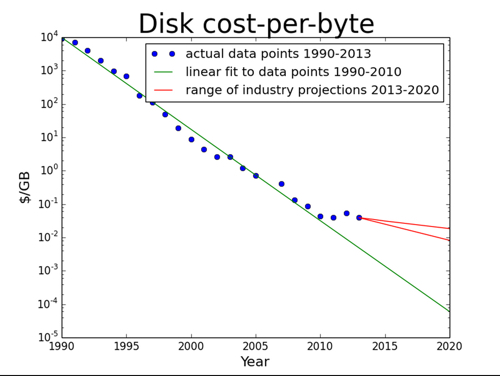
\includegraphics[width=0.75\textwidth]{img/kryder-slowdown}
\end{figure}

Een tweede kost waar er rekening mee moet worden gehouden zijn backups. Zoals vermeld in Hoofdstuk~\ref{sec:projections} zijn de databanken die gebruikt worden projecties van de afgebeelde events. Vermits deze een berekening zijn, volstaat het om enkel van de events een backup te nemen, omdat de projecties opnieuw berekend kunnen worden\footnote{Er mag niet vergeten worden om een backup te nemen van data die niet in de databank wordt opgeslagen, zoals afbeeldingen}.

Uit een gesprek met de product owner van Skedify, Christophe Thelen, bleek dat door de lage hoeveelheid data die ze nu hebben er helemaal geen problemen zijn met backups. Het is wel een interessante piste naar de toekomst toe, om enkel belangrijke data te gaan backuppen en andere data te laten berekenen, net zoals projections werken.

\subsection{Developer kosten}
\label{subsec:developer-kosten}

Het is een andere manier van werken dus zullen de developers ook op de hoogte gebracht worden hoe ze met deze technologie moeten omgaan. Er zijn verschillende resources beschikbaar, waaronder https://eventsourcery.com. Zowel bij Skedify, als bij andere bedrijven wordt er gebruik gemaakt van \gls{OOP}. EventSourcing gaat erg goed samen met functional programming omdat de huidige state een \gls{leftfold}\footnote{\glsdesc{leftfold}} is van vorige events.

\begin{equation}
\text{current state} = f(\text{events}, \text{action})
\end{equation}

Functioneel leren programmeren is dus een meerwaarde.

Bij Skedify zijn ze momenteel met een 5-tal developers, de extra kost van lessen via https://eventsourcery.com is zo klein dat ze bij Skedify hier geen probleem van maken. Het is wel zo, dat door de nieuwe en andere manier van denken er geen ruimte is om met EventSourcing te gaan werken. Dit omdat niet alle noden van de klanten gekend zijn en omdat Skedify nog zo jong in zijn schoenen staat.

\subsection{Performance kosten}
\label{subsec:performance-kosten}

Telkens wanneer er een nieuwe command uitgevoerd wordt zoals vernoemd in Hoofdstuk~\ref{subsec:imperative-messages}, moeten alle events uit de EventStore overlopen worden om de huidige staat van het object op te bouwen. Dit wil zeggen dat bij elk nieuw event, de applicatie trager zal worden. In kleine en middelmatige applicaties heeft dit geen gevolgen, naar grotere applicaties toe heeft dit grotere gevolgen. Hiervoor is een oplossing van snapshots. Een snapshot is de huidige state van een object na het overlopen van x aantal events. Deze kunnen in de EventStore opgeslagen worden, in een tabel naast de events zelf. Telkens wanneer de klasse beschrijving zou veranderen, moeten de snapshots opnieuw gegenereerd worden. Een tweede optie is om de current state ook op te slaan in memory, via deze weg moeten er geen events opnieuw afgespeeld worden om de huidige state van een object te kunnen bepalen omdat deze reeds beschikbaar is.
%%=============================================================================
%% Proof of concept
%%=============================================================================

\chapter{Proof of concept}
\label{ch:POC}

Als proof of concept worden er 2 zaken van Skedify uitgewerkt in een EventSourced systeem. Het eerste is het maken van een afspraak (appointment) en het tweede het wijzigen van een appointment (reschedulen).

De proof of concept is gemaakt in de programmeertaal PHP, dit omdat Skedify ook geschreven is in PHP. Via deze weg zitten we dichter bij de realiteit, en moeten er ook geen andere programmeertalen vergeleken worden met elkaar.

Het blijkt dat de setup van deze proof of concept zeer veel met zich mee bracht, zoals het maken van de EventStore, het bepalen van de aggregates en de Domain Events. Het is wel zo dat de \Glspl{command} en \Glspl{query} een duidelijke 1-op-1 mapping zijn met de businesskant. Dit werd als positief aanschouwd door de product owner van Skedify, Christophe Thelen.

De testbaarheid van \Glspl{command} en Domain Events gingen zeer vlot met als bonus dat er documentatie van van deze testen gegenereerd konden worden (zoals te zien in figuur~\ref{fig:documentation}).

\begin{figure}[h]
\caption{Gegenereerde documentatie van de geautomatiseerde testen} \label{fig:documentation}
\centering
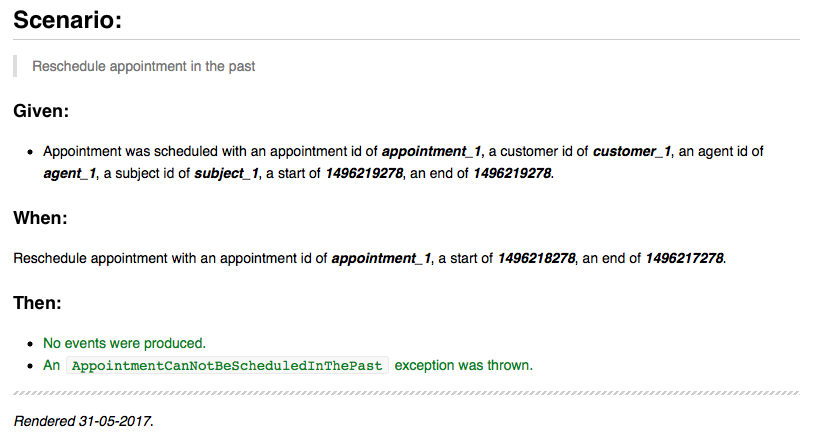
\includegraphics[width=0.9\textwidth]{img/documentatie-voorbeeld}
\end{figure}

De proof of concept kan teruggevonden worden via \textcite{malfait2017poc}.
%%=============================================================================
%% Conclusie
%%=============================================================================

\chapter{Conclusie}
\label{ch:conclusie}

%% TODO: Trek een duidelijke conclusie, in de vorm van een antwoord op de
%% onderzoeksvra(a)g(en). Wat was jouw bijdrage aan het onderzoeksdomein en
%% hoe biedt dit meerwaarde aan het vakgebied/doelgroep? Reflecteer kritisch
%% over het resultaat. Had je deze uitkomst verwacht? Zijn er zaken die nog
%% niet duidelijk zijn? Heeft het ondezoek geleid tot nieuwe vragen die
%% uitnodigen tot verder onderzoek?

Uit dit onderzoek is gebleken dat EventSourcing zeer interessant is vanuit een business standpunt. Geen data en informatie kwijtgeraken doorheen de jaren klinkt als muziek in de oren. Het opzetten van EventSourcing binnen Skedify, dat momenteel nog zeer jong is, is veel moeilijker omdat de developers opgeleid moeten worden en de noden van de klant nog niet helemaal duidelijk zijn.

Het verschil tussen EventSourcing en systemen die gebruik maken van een \gls{RDBMS} is nu ook duidelijk. Bij EventSourcing wordt er een lijst van events bijgehouden in een append only database, de EventStore. Deze events zijn ook de \gls{ssot}. De huidige staat van de applicatie wordt berekend van deze events en in een database gevoed via projections. Bij een \gls{RDBMS} is deze databank zelf de \gls{ssot}, er worden geen events in een EventStore bijgehouden. Er worden bij sommige systemen, zoals bij Skedify, wel gebruik gemaakt van een audit log.

Het bepalen van de delen die EventSourced moeten worden kan eenvoudig door te kijken naar de belangrijke core-business delen. Bij Skedify draait dit rond de afspraken, vragen en antwoorden. Meer nog, bij Skedify zouden ze, indien ze EventSourcing zouden gebruiken in de toekomst, enkel de delen rond afspraken gaan EventSourcen omdat hier de meeste vragen van hun klanten over komen.

EventSourcing biedt momenteel geen meerwaarde voor Skedify\footnote{Het is wel interessant om dit onderzoek nog eens uit te voeren over enkele jaren, wanneer het product matuurder geworden is}.

De verwachtingen waren net iets anders, er werd verwacht dat EventSourcing wel een meerwaarde zou bieden naar Skedify toe. Uit gesprekken bij Skedify, en uit het onderzoek is nu eenmaal gebleken dat dit niet het geval is.

Naar de toekomst toe kan het wel interessant zijn dit nog eens opnieuw te onderzoeken. Het kan ook interessant zijn om met dit onderzoek verder te gaan en te gaan kijken hoe er effectief van de huidige manier van werken, naar EventSourcing geëvolueerd kan worden.

%%---------- Back matter ------------------------------------------------------

\phantomsection
\printbibliography

\addcontentsline{toc}{chapter}{\textcolor{maincolor}{\IfLanguageName{dutch}{Bibliografie}{Bibliography}}}

\listoffigures
\listoftables

\end{document}
